    \subsection{Bisection Refinement in 2-dimension and its stability}
    Another popular refinement strategy is bisection. Basically, we cut a triangle by connecting one vertex, which we choose as the peak, with its opposite edge, which we call refinement edge. Generally, if we apply random bisection with no plan on a triangle, it is likely that we fail to preserve stability and consistency.

    Hence, one important part we need to consider is how to choose the peak for a triangle to preserve the stability and consistency, and one famous method was introduced as the $newest vertex$ bisection. In newest vertex bisection, we create the newest vertex at the middle of the refinement edge after applying the bisection refinement once, and then we regard the newest vertex as the peak for bisection over the resulting two smaller triangles.

    \begin{figure}[h!]
    \centering
      \begin{tikzpicture}[scale=0.7]
      \tkzDefPoint(-6.5,0){A''}
      \tkzDefPoint(-5,2){peak}
      \tkzDefPoint(-3,0){C''}
      \tkzDrawSegments(A'',peak peak,C'' A'',C'')
    %\tkzDrawSegments(A'',B'' B'',C'' A'',C'')
      \tkzLabelPoints[above,yshift=0pt](peak)
    %\tkzDefMidPoint(A'',C'') \tkzGetPoint{new vertex}
    %\tkzLabelPoints[below,yshift=0pt](new vertex)
    %\tkzDefLine[orthogonal=through ac](A,C)
    
    \tkzDefPoint(-2,0){A}
    \tkzDefPoint(-0.5,2){B}
    \tkzDefPoint(1.5,0){C}
    \tkzDrawSegments(A,B B,C A,C)
    \tkzDefMidPoint(A,B) \tkzGetPoint{peak}
    \tkzLabelPoints[left](peak)
    \tkzDefMidPoint(B,C) \tkzGetPoint{peak}
    \tkzLabelPoints[right](peak)
    \tkzDefMidPoint(A,C) \tkzGetPoint{ac}
    \tkzDefLine[orthogonal=through ac](A,C)
    \tkzDrawSegment(B,ac)


    \tkzDefPoint(2.5,0){A'}
    \tkzDefPoint(4,2){B'}
    \tkzDefPoint(6,0){C'}
    \tkzDrawSegments(A',B' B',C' A',C')
    \tkzDefMidPoint(A',B') \tkzGetPoint{ab'}
    \tkzDefLine[orthogonal=through ab'](A',B')
    \tkzDefMidPoint(A',C') \tkzGetPoint{ac'}
    \tkzDefLine[orthogonal=through ac'](A',C')
    \tkzDefMidPoint(B',C') \tkzGetPoint{bc'}
    \tkzDefLine[orthogonal=through bc'](B',C')
    \tkzDrawSegment(B',ac')
    \tkzDrawSegment(ac',ab')
    \tkzDrawSegment(ac',bc')
    \tkzDefMidPoint(B',ac') \tkzGetPoint{peak}
    \tkzLabelPoints[above,yshift=0pt](peak)
    \tkzDefMidPoint(A',ac') \tkzGetPoint{peak}
    \tkzLabelPoints[below](peak)
    \tkzDefMidPoint(C',ac') \tkzGetPoint{peak}    
    \tkzLabelPoints[below](peak)


    \tkzDefPoint(7,0){A'''}
    \tkzDefPoint(8.5,2){B'''}
    \tkzDefPoint(10.5,0){C'''}
    \tkzDrawSegments(A''',B''' B''',C''' A''',C''')
    \tkzDefMidPoint(A''',B''') \tkzGetPoint{ab''}
    \tkzDefLine[orthogonal=through ab''](A''',B''')
    \tkzDefMidPoint(A''',C''') \tkzGetPoint{ac''}
    \tkzDefLine[orthogonal=through ac''](A''',C''')
    \tkzDefMidPoint(B''',C''') \tkzGetPoint{bc''}
    \tkzDefLine[orthogonal=through bc''](B''',C''')
    \tkzDrawSegment(B''',ac'')
    \tkzDrawSegment(ac'',ab'')
    \tkzDrawSegment(ac'',bc'')
    \tkzDefMidPoint(B''',ac'') \tkzGetPoint{x}
    \tkzDefLine[orthogonal=through x](B''',ac'')
    \tkzDefMidPoint(A''',ac'') \tkzGetPoint{y}
    \tkzDefLine[orthogonal=through y](A''',ac'')
    \tkzDefMidPoint(C''',ac'') \tkzGetPoint{z}
    \tkzDefLine[orthogonal=through z](C''',ac'')
    \tkzDrawSegment(ab'',x)
    \tkzDrawSegment(bc'',x)
    \tkzDrawSegment(ab'',y)
    \tkzDrawSegment(bc'',z)
    \end{tikzpicture}
    \caption{Illustration of bisection refinement, starting with a single triangle}
    \label{Fig4}
    \end{figure}







%----------------------------------------------------------------------------------
    %\subsection{Stability of Newest Vertex Bisection}
    \begin{lemma*}
    Bisection refinement gives four congruence classes given one triangle.
    \end{lemma*}
    \begin{proof}
    \begin{figure}[h!]
    \centering
      \begin{tikzpicture}[scale=0.8]
      \tkzDefPoint(-9,0){A''}
      \tkzDefPoint(-7.5,2){B''}
      \tkzDefPoint(-5.5,0){C''}
      \tkzDrawSegments(A'',B'' B'',C'' A'',C'')
      \node (t) at (-7.5, 1) {{1}};

      \tkzDefPoint(-2,0){A}
      \tkzDefPoint(-0.5,2){B}
      \tkzDefPoint(1.5,0){C}
      \tkzDrawSegments(A,B B,C A,C)
      \tkzDefMidPoint(A,C) \tkzGetPoint{ac}
      \tkzDefLine[orthogonal=through ac](A,C)
      \tkzDrawSegment(B,ac)
      \node (t') at (-1, 0.5) {{2}};
      \node (t'') at (0.5, 0.5) {{3}};
      \end{tikzpicture}
    \caption{Stage 1: Original triangle(left); Stage 2: Applied the newest vertex bisection once(right)}
    \label{fig5: sub1}
    \end{figure}

    Observing Figure 5, we have a triangle at the beginning, say it's in congruency class 1. After applying the newest vertex bisection refinement once, we obtain two smaller pieces of triangles as in the second picture in Figure 5. Say one of them is in congruency class 2, and another one is in congruency class 3. Further applying the newest vertex bisection refinement, we have the figures below.

    \begin{figure}[h!]
    \centering
      \begin{tikzpicture}[scale=0.8] 
      \tkzDefPoint(0,0){A'}
      \tkzDefPoint(1.5,2){B'}
      \tkzDefPoint(3.5,0){C'}
      \tkzDrawSegments(A',B' B',C' A',C')
      \tkzDefMidPoint(A',B') \tkzGetPoint{ab'}
      \tkzDefLine[orthogonal=through ab'](A',B')
      \tkzDefMidPoint(A',C') \tkzGetPoint{ac'}
      \tkzDefLine[orthogonal=through ac'](A',C')
      \tkzDefMidPoint(B',C') \tkzGetPoint{bc'}
      \tkzDefLine[orthogonal=through bc'](B',C')
      \tkzDrawSegment(B',ac')
      \tkzDrawSegment(ac',ab')
      \tkzDrawSegment(ac',bc')
      \node (t''') at (1.2, 1) {{4}};
      \node (t''') at (2, 1) {{4}};
      \node (t) at (0.8, 0.5) {{1}};
      \node (t) at (2.5, 0.5) {{1}};

      \tkzDefPoint(7,0){A'''}
      \tkzDefPoint(8.5,2){B'''}
      \tkzDefPoint(10.5,0){C'''}
      \tkzDrawSegments(A''',B''' B''',C''' A''',C''')
      \tkzDefMidPoint(A''',B''') \tkzGetPoint{ab''}
      \tkzDefLine[orthogonal=through ab''](A''',B''')
      \tkzDefMidPoint(A''',C''') \tkzGetPoint{ac''}
      \tkzDefLine[orthogonal=through ac''](A''',C''')
      \tkzDefMidPoint(B''',C''') \tkzGetPoint{bc''}
      \tkzDefLine[orthogonal=through bc''](B''',C''')
      \tkzDrawSegment(B''',ac'')
      \tkzDrawSegment(ac'',ab'')
      \tkzDrawSegment(ac'',bc'')
      \tkzDefMidPoint(B''',ac'') \tkzGetPoint{x}
      \tkzDefLine[orthogonal=through x](B''',ac'')
      \tkzDefMidPoint(A''',ac'') \tkzGetPoint{y}
      \tkzDefLine[orthogonal=through y](A''',ac'')
      \tkzDefMidPoint(C''',ac'') \tkzGetPoint{z}
      \tkzDefLine[orthogonal=through z](C''',ac'')
      \tkzDrawSegment(ab'',x)
      \tkzDrawSegment(bc'',x)
      \tkzDrawSegment(ab'',y)
      \tkzDrawSegment(bc'',z)
      \node (t') at (7.5, 0.3) {{2}};
      \node (t'') at (8.2, 0.3) {{3}};
      \node (t'') at (8.4, 0.7) {{3}};
      \node (t') at (8.3, 1.4) {{2}};
      \node (t'') at (8.9, 1.4) {{3}};
      \node (t') at (8.9, 0.7) {{2}};
      \node (t') at (9.3, 0.3) {{2}};
      \node (t'') at (9.8, 0.3) {{3}};
      \end{tikzpicture}
    \caption{Stage 3: Applied the newest vertex bisection twice(left); Stage 4: Applied the newest vertex bisection three times(right)}
    \label{fig5: sub2}
    \end{figure}

    \begin{claim}
    The left and right bottom triangles in Stage 3 are congruent to the original triangle in Stage 1, and they are in the congruency class 1. Moreover, the other two triangles left are congruent and in congruency class 4.
    \end{claim}
    %\begin{proof}\mbox{}\\
    \noindent
    Proof of Claim 1: \\
    Let A, B, C be the vertices of the triangle $T$ and let X, Y, Z be the midpoints of the edge AB, AC and BC. An application of the newest vertex bisection refinement produces the triangle $\triangle{AXY}, \triangle{XBY}, \triangle{ZBY}$ and $\triangle{YZC}$. Consider the Fig 8 (left).
    Since X, Y, Z be the midpoints of the edge AB, AC and BC, we have 
    \begin{align*}
     XY \parallel BC,
     \quad 
     ZY \parallel AB,
     \quad 
     AX = BX, 
     \quad 
     BZ = CZ, 
     \quad
     AY = CY
    \end{align*}
    Since $XY\parallel BC$, we have $\angle{AXY} = \angle{ABC}$ and $\angle{XYB} = \angle{ZBY}$. Similarly, since $ZY\parallel AB$, we have $\angle{YZC} = \angle{ABC}$ and $\angle{XBY} = \angle{ZYB}$. Thus 
    \begin{align*}
    \angle{XYB} = \angle{ZBY},
    \quad
    |BY| = |BY|,
    \quad
    \angle{XBY} &= \angle{ZYB}.
    \end{align*}
    Therefore, we have $\triangle{XBY} \cong \triangle{ZYB}$, and we mark them in the congruency class 4. This further gives us $|AX| = |BX| = |YZ|$, and $|ZC| = |BZ| = |XY|$.
    \begin{align*}
    |AX| = |YZ|,
    \quad
    \angle{AXY} = \angle{ABC} = {YZC},
    \quad
    |XY| = |ZC|.
    \end{align*}
    Therefore, we have $\triangle{AXY} \cong \triangle{YZC}$. It's clear that $\triangle{AXY}$ and $\triangle{YZC}$ are similar to $\triangle{ABC}$ as all their angles are the same. Thus, we finished the proof of claim 1.

    %\end{proof}%end proof of claim 1

    \begin{claim}
    Triangles with same number in Stage 4 in a same congruency class marked by the number.
    \end{claim}
    %\begin{proof}
    \noindent
    Proof of Claim 2: \\
    Let A, B, C be the vertices of the triangle $T$ and let X, Y, Z be the midpoints of the edge AB, AC and BC, and M, N, P be the midpoints of the edge AY, CY and BY. Consider the Fig 8 (right).
 
    An application of the newest vertex bisection refinement produces the following triangles
    \begin{align*}
    \triangle{AXM}, \triangle{XBP}, \triangle{ZYP}, \triangle{YZN}, \triangle{MXY}, \triangle{PBZ}, \triangle{PYX}, \triangle{NZC}
    \end{align*}
    Notice that X, P and Z are three points one a stright line. This is clear because $XP\parallel AY$ and $PZ\parallel YC$, and we have $\angle{BPX}+\angle{BPZ} = \angle{BYA}+\angle{BYC} = \pi$. Basically, to prove the Stage 4 is equivalent to prove the following
    \begin{align*}
    \triangle{AXM}\cong\triangle{XBP}\cong\triangle{ZYP}\cong\triangle{YZN}\\
    \triangle{MXY}\cong\triangle{PBZ}\cong\triangle{PYX}\cong\triangle{NZC}
    \end{align*}
    Similarily to proof of Claim 1, we have
    \begin{align*}
    XY\parallel BC,
    \quad
    YZ\parallel AB,
    \quad
    XZ\parallel AC,
    \quad
    XM\parallel BY\parallel ZN
    \end{align*}
    Therefore, we further have 
    \begin{align*}
    \angle{BAY} = \angle{ZYC},
    \quad
    \angle{BCY} = \angle{XYA},
    \quad
    \angle{AXC} = \angle{ABC} = \angle{YZC}\\
    \angle{PZY} = \angle{ZYN},
    \quad
    \angle{PYZ} = \angle{NZP},
    \quad
    \angle{PXY} = \angle{XYM},
    \quad
    \angle{PYX} = \angle{MXY},
    \end{align*}
    Then it is clear that
    \begin{align*}
    \triangle{AXY} \sim \triangle{ABC} \sim \triangle{YZC}
    \end{align*}
    Similarly, we can find that 
    \begin{align*}
    \triangle{XBZ}\sim\triangle{ABC},
    \quad
    \triangle{AXM}\sim\triangle{ABY},
    \quad
    \triangle{CZN}\sim\triangle{CBY}.
    \end{align*}
    In other words, 
    \begin{align*}
    \triangle{AXM}\sim\triangle{ABY}\sim\triangle{XBP}\sim\triangle{YZN},\\
    \triangle{CZN}\sim\triangle{CBY}\sim\triangle{YXM}\sim\triangle{ZBP}.
    \end{align*}
    Moreover, since the ratio of $\|AX\|, \|BX\|$, and $\|ZY\|$ is 1, and the ratio of $\|ZC\|, \|BZ\|$, and $\|XY\|$ is 1, we have
    \begin{align*}
    \triangle{AXM}\cong\triangle{XBP}\cong\triangle{YZN},\\
    \triangle{CZN}\cong\triangle{YXM}\sim\triangle{ZBP}.
    \end{align*}
    Therefore, we showed that $\triangle{AXM}, \triangle{XBP}$ and $\triangle{YZN}$ are in congruency class 2, and $\triangle{CZN}, \triangle{YXM}$ and $\triangle{ZBP}$ are in congruency class 3.
    Moreover, since 
    \begin{align*}
    \angle{PZY} = \angle{ZYN},
    \quad
    \angle{PYZ} = \angle{NZP},
    \quad
    \angle{PXY} = \angle{XYM},
    \quad
    \angle{PYX} = \angle{MXY},
    \end{align*}
    we have that
    \begin{align*}
    \triangle{YZN}\cong\triangle{YZP},
    \quad
    \triangle{YXM}\cong\triangle{YXP}.
    \end{align*}
    Therefore we proved 
    \begin{align*}
    \triangle{AXM}\cong\triangle{XBP}\cong\triangle{ZYP}\cong\triangle{YZN}\sim\triangle{ABY},\\
    \triangle{MXY}\cong\triangle{PBZ}\cong\triangle{PYX}\cong\triangle{NZC}\sim\triangle{YBC}.
    \end{align*}
    %\end{proof}
    Thus, we finished proof of Claim 2.
    
    %------------------------------------------------------------------------
    %figure for claims proof
    \begin{figure}[h!]
    \centering
    \begin{tikzpicture}[scale=0.8]
    \tkzDefPoint(-4.5,0){A}
    \tkzDefPoint(-3,2){B}
    \tkzDefPoint(-1,0){C}
    \tkzDrawSegments(A,B B,C A,C)
    \tkzLabelPoints[left](A)
    \tkzLabelPoints[above](B)
    \tkzLabelPoints[right](C)
    \tkzDefMidPoint(A,B) \tkzGetPoint{X}
    \tkzDefLine[orthogonal=through X](A,B)
    \tkzDefMidPoint(A,C) \tkzGetPoint{Y}
    \tkzDefLine[orthogonal=through Y](A,C)
    \tkzDefMidPoint(B,C) \tkzGetPoint{Z}
    \tkzDefLine[orthogonal=through Z](B,C)
    \tkzDrawSegment(B,Y)
    \tkzDrawSegment(Y,X)
    \tkzDrawSegment(Y,Z)
    \tkzLabelPoints[above, xshift=-2mm](X)
    \tkzLabelPoints[above, xshift=2mm](Z)
    \tkzLabelPoints[below,yshift=0pt](Y)

    \tkzDefPoint(2.5,0){A}
    \tkzDefPoint(4,2){B}
    \tkzDefPoint(6,0){C}
    \tkzDrawSegments(A,B B,C A,C)
    \tkzLabelPoints[left](A)
    \tkzLabelPoints[above](B)
    \tkzLabelPoints[right](C)
    \tkzDefMidPoint(A,B) \tkzGetPoint{X}
    \tkzDefLine[orthogonal=through X](A,B)
    \tkzDefMidPoint(A,C) \tkzGetPoint{Y}
    \tkzDefLine[orthogonal=through Y](A,C)
    \tkzDefMidPoint(B,C) \tkzGetPoint{Z}
    \tkzDefLine[orthogonal=through Z](B,C)
    \tkzDrawSegment(B,Y)
    \tkzDrawSegment(Y,X)
    \tkzDrawSegment(Y,Z)
    \tkzLabelPoints[above, xshift=-2mm](X)
    \tkzLabelPoints[above, xshift=2mm](Z)
    \tkzLabelPoints[below,yshift=0pt](Y)

    \tkzDefMidPoint(B,Y) \tkzGetPoint{P}
      \tkzDefLine[orthogonal=through P](B,Y)
      \tkzDefMidPoint(A,Y) \tkzGetPoint{M}
      \tkzDefLine[orthogonal=through M](A,Y)
      \tkzDefMidPoint(C,Y) \tkzGetPoint{N}
      \tkzDefLine[orthogonal=through N](C,Y)
      \tkzDrawSegment(X,P)
      \tkzDrawSegment(Z,P)
      \tkzDrawSegment(X,M)
      \tkzDrawSegment(Z,N)
      \tkzLabelPoints[below, xshift=-2mm](M)
    \tkzLabelPoints[below, xshift=2mm](N)
    \tkzLabelPoints[above,yshift=0pt](P)
    \end{tikzpicture}
    \caption{Illustration of newest vertex bisection for Claim 1(left); Claim 2(right)}
    \end{figure}



    Notice that in Stage 3, we see triangles in congruency class 1 again, so we can tell further applying the newest vertex bisection refinement will lead to the same process as what we have for Stage 1. Similarly, further applying the newest vertex bisection refinement over triangles in congruency class 4, 2 and 3 are already explored in Stage 3 and 4. Therefore, we actually obtain 4 congruency classes only.
    \end{proof}
    This means that we never have triangles degenerating when applying the newest vertex bisection refinement, because the number of congruence classes is four, which is finite, and by theorem proved in 3.1, we see that the newest vertex bisection refinement strategy is stable.

    As we explain in section 3, a good refinement strategy should preserve both stability and consistency. Before we take a look at consistency, let's first introduce dependency graph.

    \subsection{Compatible Divisibility and Consistency}
    \begin{definition*}
      Let G = (V, E) be a directed graph, where V represents triangles, and $(V_1, V_2)\in E$ if the refinement edge of $v_1$ neighbors at $v_2$, and then we call G a dependency graph.
      \begin{align*}
      V &= \{Triangles\}\\
      E &= \{(V_1, V_2)\in V\times V | \text{The refinement edge of $V_1$ neighbors $V_2$}\}
      \end{align*}
    \end{definition*}
    Note that $V$ and $E$ in this definition are quite different from general geometry, and all nodes of one dependency graph have at most one outgoing edge (See Figure 9).%[Multiple V's, graph? need proof???]
    \begin{figure}[h!]
    \centering
    \begin{tikzpicture}[scale=0.8]
    \tkzDefPoint(0.5,0.1){A}
    \tkzDefPoint(3,0.5){B}
    \tkzDefPoint(1.7,2.7){C}
    \tkzDrawSegments(A,B B,C A,C)

    \tkzDefPoint(2,2.8){A'}
    \tkzDefPoint(3.3,0.6){B'}
    \tkzDefPoint(4.8,3){C'}
    \tkzDrawSegments(A',B' B',C' A',C')

    \tkzDefPoint(2.22,2.75){X}
    \tkzDefPoint(3.4,0.72){Y}
    \tkzDrawSegment[thick, color=red](X, Y)
    \draw [blue,  ->   ] (3.35,2.2) -- (1.2,0.7);
    \end{tikzpicture}
    \caption{Illustration of outgoing arrow in dependency graph}
    \label{Figure 9}
    \end{figure}


    \begin{definition*}
      A triangle is called compatibly divisible if either
      \begin{itemize}
        \item[a. ] it has no outgoing edge in G
        \item[b. ] it is part of a cycle in G whose size is 2.
      \end{itemize}
    \end{definition*}
    \begin{figure}[h!]
    \centering
    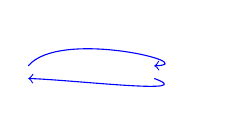
\begin{tikzpicture}[scale=0.8]
    \tkzDefPoint(-4,0){A}
    \tkzDefPoint(-3,2){B}
    \tkzDefPoint(-2,0){C}
    \tkzDrawSegments(A,B B,C A,C)
    \tkzDefPoint(-6,2.2){D}
    \tkzDrawSegments(A,D B,D)
    \tkzDefPoint(-1,1){E}
    \tkzDrawSegments(C,E B,E)
    %\tkzDefPoint(-5,0.5){F}
    %\tkzDrawSegments(A,F)
    %\tkzDefPoint(-1.5,0){G}
    %\tkzDrawSegments(C,G)
    \tkzDefPoint(-4.1,-0.1){X}
    \tkzDefPoint(-1.9,-0.1){Y}
    \tkzDrawSegment[thick, color=red](X, Y)

    \tkzDefPoint(3,1.5){A'}
    \tkzDefPoint(5,0){B'}
    \tkzDefPoint(5,3){C'}
    \tkzDrawSegments(A',B' B',C' A',C')
    \tkzDefPoint(7,2){D'}
    \tkzDrawSegments(B',D' C',D')
    \tkzDefPoint(4.9,0.1){X'}
    \tkzDefPoint(4.9,2.9){Y'}
    \tkzDefPoint(5.1,0.1){M'}
    \tkzDefPoint(5.1,2.9){N'}
    \tkzDrawSegment[thick, color=red](X', Y')
    \tkzDrawSegment[thick, color=red](M', N')

    \draw [->, blue] (4, 1.6) to [out=50,in=2] (6, 1.6);
    \draw [->, blue] (6, 1.4) to [out=-20,in=-2] (4, 1.4);
    \end{tikzpicture}
    \caption{Compatibly divisible triangles: case a(left); case b(right)}
    \label{Figure 10}
    \end{figure}
    Triangles of case b in Figure above are called mates as they share same refinement edge in 2-cycle.

    \noindent
    {Compatible divisibility in Dependency Graph}
    \begin{figure}[h!]
    \centering
    \begin{tikzpicture}[scale=0.5]
    \tkzDefPoint(2,2.5){A}
    \tkzDefPoint(5,0){B}
    \tkzDefPoint(5,3){C}
    \tkzDrawSegments(A,B B,C A,C)
    \tkzDefPoint(8,2){D}
    \tkzDrawSegments(B,D C,D)
    \tkzDefPoint(1,-1){E}
    \tkzDrawSegments(A,E B,E)
    \tkzDefPoint(3,-3){F}
    \tkzDrawSegments(E,F B,F)

    \tkzDefPoint(5.1,2.9){X}
    \tkzDefPoint(5.1,0.1){Y}
    \tkzDrawSegment[thick, color=red](X, Y)
    \tkzDefPoint(2.2, 2.5){X'}
    \tkzDefPoint(4.9, 0.3){Y'}
    \tkzDrawSegment[thick, color=red](X', Y')
    \tkzDefPoint(1.1,-0.8){M}
    \tkzDefPoint(4.8,0.1){N}
    \tkzDrawSegment[thick, color=red](M, N)
    \tkzDefPoint(1.15,-1.1){M'}
    \tkzDefPoint(4.8,-0.2){N'}
    \tkzDrawSegment[thick, color=red](M', N')

    \draw [blue,  ->   ] (6,1.5) -- (4.5,1.7);
    \draw [blue,  ->   ] (4,1.7) -- (3,1);
    \draw [->, blue] (2.6, 0.5) to [out=50,in=2] (2.9, -1.5);
    \draw [->, blue] (2.8, -1.5) to [in=2,out=20] (2.5, 0.5);


    \tkzDefPoint(10,2.5){A}
    \tkzDefPoint(13,0){B}
    \tkzDefPoint(13,3){C}
    \tkzDrawSegments(A,B B,C A,C)
    \tkzDefPoint(16,2){D}
    \tkzDrawSegments(B,D C,D)
    \tkzDefPoint(9,-1){E}
    \tkzDrawSegments(A,E B,E)
    \tkzDefPoint(11,-3){F}
    \tkzDrawSegments(E,F B,F)

    \tkzDefPoint(13.1,2.9){X}
    \tkzDefPoint(13.1,0.1){Y}
    \tkzDrawSegment[thick, color=red](X, Y)
    \tkzDefPoint(10.2, 2.5){X'}
    \tkzDefPoint(12.9, 0.3){Y'}
    \tkzDrawSegment[thick, color=red](X', Y')

    \tkzDefPoint(10.1,2.2){M}
    \tkzDefPoint(12.6,0.1){N}
    \tkzDrawSegment[thick, color=red](M, N)
    \tkzDefPoint(9.2,-0.9){M'}
    \tkzDefPoint(10.1,2.2){N'}
    \tkzDrawSegment[thick, color=red](M', N')

    \tkzDefPoint(9.3,-1.1){K}
    \tkzDefPoint(11,-2.8){L}
    \tkzDrawSegment[thick, color=red](K, L)
    \tkzDefPoint(12.75,-0.1){K'}
    \tkzDefPoint(11,-2.8){L'}
    \tkzDrawSegment[thick, color=red](K', L')

    \draw [blue,  ->   ] (14,1.5) -- (12.5,1.7);
    \draw [blue,  ->   ] (12.2,1.4) to [out=50,in=2] (11,0.7);
    \draw [blue,  ->   ] (10.9,0.9) to [out=50,in=2] (12,1.7);
    %\draw [->, blue] (10.6, 0.5) to [out=50,in=2] (10.9, -1.5);
    %\draw [->, blue] (10.8, -1.5) to [in=2,out=20] (10.5, 0.5);
    \end{tikzpicture}
    \caption{Compatible divisibility in Dependency Graph}
    \end{figure}
    In Figure 11, we see a compatibility chain in a triangulation. When performing the newest vertex bisection on the right most triangle, we need to bisect its left neighboring triangle first. We obtain a recursion here since we need to bisect the triangle which our current target triangle depends on. If we successfully reached the base case, either on boundary or a cycle of size 2, we can then bisect back in an order like stack. In the example displayed in Figure 11, a base case is reached by bisecting the left most two triangles. However, a base case is not always promised. In other word, it is not guaranteed that we can always achieve either bisection on the boundary or a cycle of size 2. One example is displayed in Figure 12, and this failed in applying the newest vertex bisection, because smaller triangles are dependent on each other. That is, its dependency graph is a cycle instead of a forest, i.e. collection of trees.

    \begin{figure}[h!]
    \centering
    %\newdimen\R
    %\R=0.8cm
    \usetikzlibrary{calc}
\tikzset{
parallel segment/.style={
   segment distance/.store in=\segDistance,
   segment pos/.store in=\segPos,
   segment length/.store in=\segLength,
   to path={
   ($(\tikztostart)!\segPos!(\tikztotarget)!\segLength/2!(\tikztostart)!\segDistance!90:(\tikztotarget)$) -- 
   ($(\tikztostart)!\segPos!(\tikztotarget)!\segLength/2!(\tikztotarget)!\segDistance!-90:(\tikztostart)$)  \tikztonodes
   }, 
   % Default values
   segment pos=.5,
   segment length=18ex,
   segment distance=1mm,
},
}
    \begin{tikzpicture}[scale=0.8]
    %\draw (0:\R) \foreach \x in {60,120,...,359} {
    %            -- (\x:\R)
     %}-- cycle (90:\R) node[above] {$n=6$} ;

    \coordinate (A) at (0,0);
    \coordinate (B) at (3,0);
    \tkzDefEquilateral(B,A)\tkzGetPoint{C};
    \tkzDrawPolygon(A,B,C);
    \tkzDefEquilateral(C,A)\tkzGetPoint{D};
    \tkzDrawPolygon(A,C,D);
    \tkzDefEquilateral(C,D)\tkzGetPoint{E};
    \tkzDrawPolygon(E,C,D);
    \tkzDefEquilateral(C,E)\tkzGetPoint{F};
    \tkzDrawPolygon(C,E,F);
    \tkzDefEquilateral(C,F)\tkzGetPoint{G};
    \tkzDrawPolygon(C,F,G);
    \tkzDefEquilateral(C,G)\tkzGetPoint{H};
    \tkzDrawPolygon(C,G,H);

    \draw[red] (A) to[parallel segment] (C);
    \draw[red] (D) to[parallel segment] (C);
    \draw[red] (E) to[parallel segment] (C);
    \draw[red] (F) to[parallel segment] (C);
    \draw[red] (G) to[parallel segment] (C);
    \draw[red] (B) to[parallel segment] (C);

    \tkzDefLine[orthogonal=through L](B,C) \tkzGetPoint{bc}
    \tkzDefLine[orthogonal=through L](A,C) \tkzGetPoint{ac}
    \tkzDefLine[orthogonal=through L](D,C) \tkzGetPoint{dc}
    \tkzDefLine[orthogonal=through L](E,C) \tkzGetPoint{ec}
    \tkzDefLine[orthogonal=through L](F,C) \tkzGetPoint{fc}
    \tkzDefLine[orthogonal=through L](G,C) \tkzGetPoint{gc}
    \end{tikzpicture}
    \caption{Failure of applying newest vertex bisection}
    \end{figure}


    \begin{lemma*}
    If the newest vertex bisection is only performed on 
    \begin{itemize}
        \item[a. ] triangles isolated in the dependency graph
        \item[b. ] pairs of mates
      \end{itemize}
    then the refinement is stable and the triangulations will be consistent.
    \end{lemma*}
    \begin{proof}
    We already proved stability in general in 2 dimension, and this applies here as well under a more strict condition. The consistency is obvious in compatibility divisible triangles.
    \end{proof}